\documentclass[12pt, letterpaper, twoside]{article}
\usepackage{nopageno,epsfig, amsmath, amssymb}
\usepackage{physics}
\usepackage{mathtools}
\usepackage{hyperref}
\usepackage{xcolor}
\hypersetup{
    colorlinks,
    linkcolor={blue},
    citecolor={blue},
    urlcolor={blue}
}
\usepackage{empheq}

\usepackage[letterpaper,
            margin=0.8in]{geometry}

\title{Astro 531; Problem Set 1}
\author{\textbf{Tom Wagg}}

\newcommand{\question}[1]{{\noindent \it #1}}
\newcommand{\answer}[1]{
    \par\noindent\rule{\textwidth}{0.4pt}#1\vspace{0.5cm}
}
\newcommand{\todo}[1]{{\color{red}\begin{center}TODO: #1\end{center}}}

% custom function for adding units
\makeatletter
\newcommand{\unit}[1]{%
    \,\mathrm{#1}\checknextarg}
\newcommand{\checknextarg}{\@ifnextchar\bgroup{\gobblenextarg}{}}
\newcommand{\gobblenextarg}[1]{\,\mathrm{#1}\@ifnextchar\bgroup{\gobblenextarg}{}}
\makeatother

\newcommand{\avg}[1]{\left\langle #1 \right\rangle}
\newcommand{\angstrom}{\mbox{\normalfont\AA}}
\allowdisplaybreaks

\begin{document}

\maketitle

\question{\textbf{2.1 - Stellar Properties}}

\question{Part a - Radi  us}
\answer{
    \begin{align}
        L &= 4 \pi R^2 \sigma T_{\rm eff}^4 \\
        R &= \sqrt{\frac{L}{4 \pi \sigma T_{\rm eff}^4}} \\
        \Aboxed{ R &= 2570 \unit{R_{\odot}} }
    \end{align}
}

\question{Part b - Density}
\answer{
    If we assume that the star is a constant density throughout then we can use the definition of density and the radius we calculated above.
    \begin{align}
        \rho &= \frac{M}{\frac{4}{3} \pi R^3} \\
        \Aboxed{ \rho &= 1.66 \times 10^{-6} \unit{kg}{m^{-3}} }
    \end{align}
}

\question{Part c - Escape velocity}
\answer{
    \begin{equation}
        \boxed{ v_{\rm esc} = \sqrt{ \frac{2 G M}{R} } = 54500 \unit{m}{s^{-1}} }
    \end{equation}
}

\question{Part d - Comparisons to Sun}
\answer{
    This star is clearly much larger than the sun (by a factor of 2570) but is \textbf{much} less dense (since the mean density of the sun is approximately $1400 \unit{kg}{m^{-3}}$, so the density is $10^{9}$ times lower than the sun). Finally, the escape velocity is lower than the sun (around 0.088 times lower). 
}

\pagebreak

\question{\textbf{3.5 - Kepler's 3rd Law from Virial Theorem}}
\answer{
    The virial theorem gives the following relations between energies
    \begin{equation}
        E_{\rm kin} = - \frac{1}{2} E_{\rm pot}
    \end{equation}
    For the orbits of planets around the sun, their potential energy will come from the gravitational potential and so
    \begin{equation}
        E_{\rm pot} = - \frac{G m_1 m_2}{a},
    \end{equation}
    and the kinetic energy is simply
    \begin{equation}
        E_{\rm kin} = \frac{1}{2} m_1 v_1^2 + \frac{1}{2} m_2 v_2^2.
    \end{equation}
    For the next part, it will be useful to define the distance from each body to the centre of mass, $a_i$, in terms of the masses
    \begin{equation}
        a_i = \frac{a \cdot m_{1 - i}}{m_1 + m_2} \\
    \end{equation}
    and additionally, it's useful to write the velocity in terms of the period and masses
    \begin{align}
        v_i &= \frac{2 \pi a_i}{P} \\
        v_i &= \frac{2 \pi}{P} \frac{a \cdot m_{1 - i}}{m_1 + m_2}
    \end{align}
    Now we can put this all together in the expression for the virial theorem.
    \begin{align}
        \frac{1}{2} m_1 v_1^2 + \frac{1}{2} m_2 v_2^2 &= \frac{1}{2} \cdot \frac{G m_1 m_2}{a}, \\
        \frac{1}{2} m_1 \qty(\frac{2 \pi}{P} \frac{a \cdot m_2}{m_1 + m_2})^2 + \frac{1}{2} m_2  \qty(\frac{2 \pi}{P} \frac{a \cdot m_1}{m_1 + m_2})^2 &= \frac{G m_1 m_2}{2 a} \\
        \frac{2 \pi^2 a^2}{P^2 M^2} \qty( m_1 m_2^2 + m_2 m_1^2 ) &= \frac{G m_1 m_2}{2 a} \\
        \frac{a^3}{P^2} &= \frac{G}{4 \pi^2} \frac{M^2 m_1 m_2}{\qty( m_1 m_2^2 + m_2 m_1^2 )} \\
        \frac{a^3}{P^2} &= \frac{G}{4 \pi^2} \frac{M^2}{\qty( m_1 + m_2 )} \\
        \Aboxed{ \frac{a^3}{P^2} &= \frac{G M}{4 \pi^2} }
    \end{align}
}

\pagebreak

\question{\textbf{4.4 - Central Temperature-Density}}
\answer{
    Here's a plot of the three different stars on (pretty much) the same figure as the textbook (I made the boundaries using Onno Pols' lecture notes but shaded them the same way as the textbook). I've also indicated the main sequence turnoff and the exhaustion of central helium as dots in the tracks (where the tracks evolve from the bottom left to top right).
    \begin{center}
        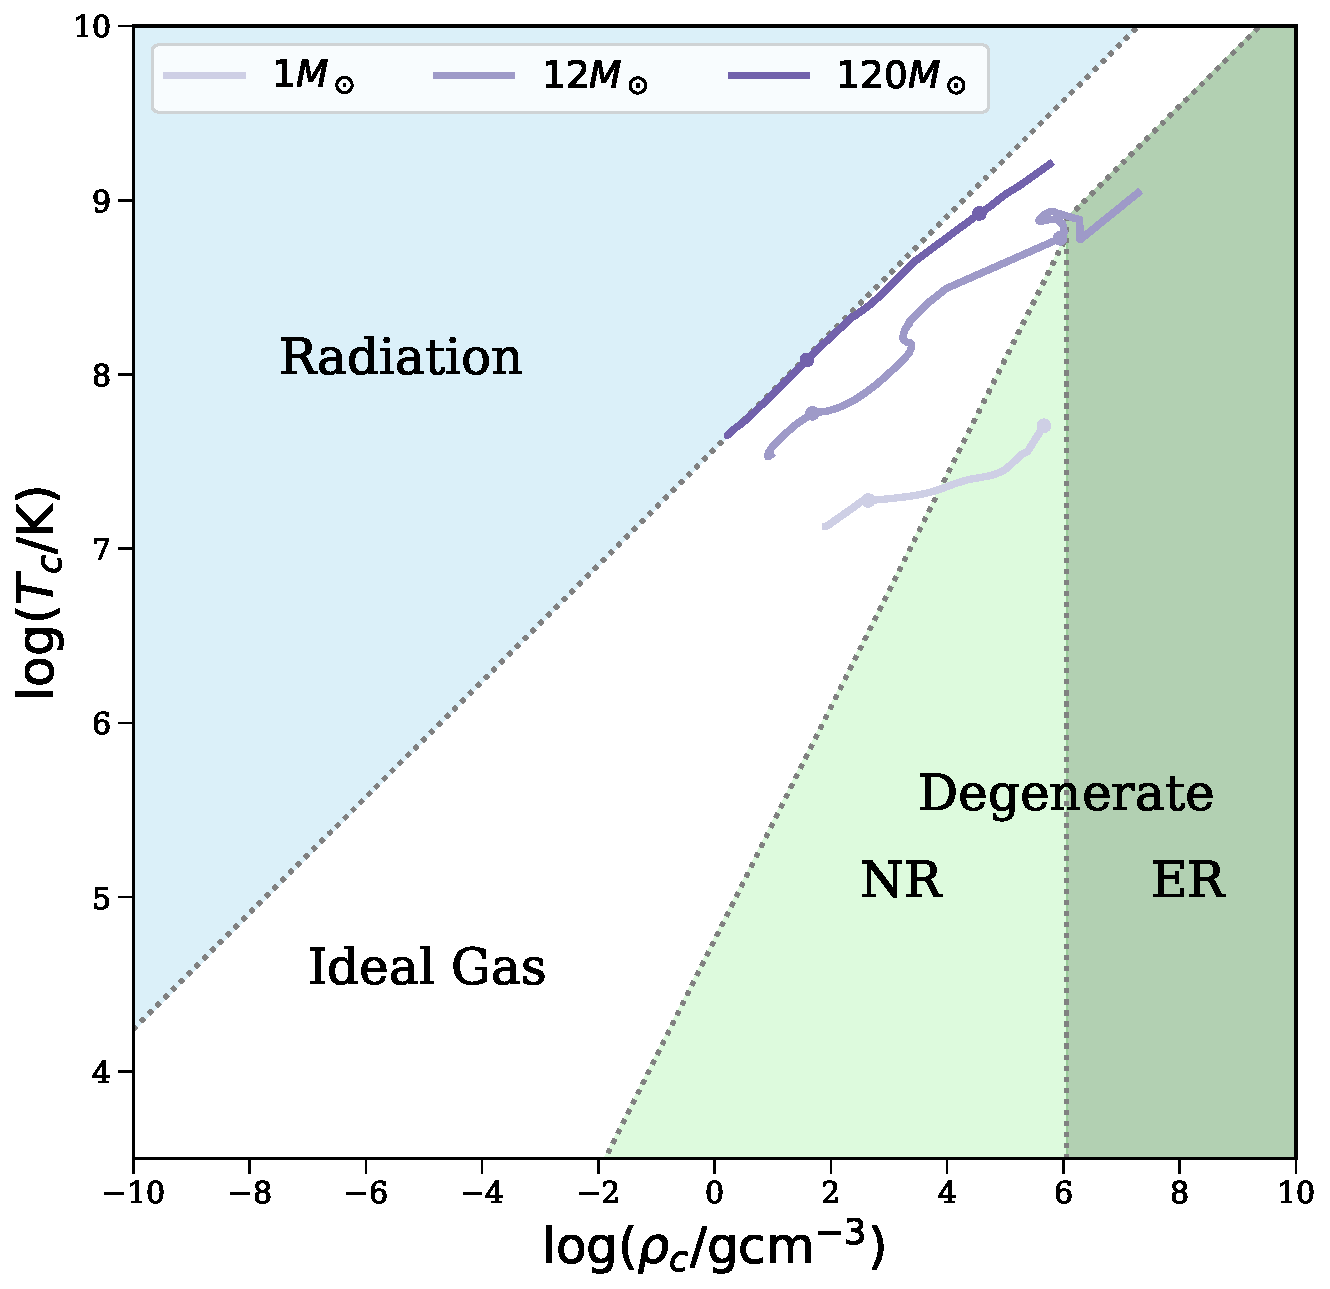
\includegraphics[width=0.8\textwidth]{figures/central_T_rho.pdf}
    \end{center}
    From these tracks we can conclude that over time each of the stars is increasing in temperature and density within its core. For the $1 \unit{M_{\odot}}$ star, it moves from the ideal gas regime to the degenerate (but non-relativistic) regime during core helium burning. This makes sense as the core of the star at this stage would be a white dwarf, despite it still being ``living'' in the outer later.

    The $12 \unit{M_{\odot}}$ star remains in the ideal gas regime all the way up until central helium exhaustion. Once helium is exhausted in the core, the star drifts into the extremely relativistic degenerate regime. This makes sense as we would expect this star to end its life as a neutron star.

    Finally, the $120 \unit{M_{\odot}}$ star very closely follows the radiation-ideal gas boundary, particularly during its main sequence. After this it moves more clearly into the ideal gas regime and, though it appears to end its life here, the models only evolve through carbon burning. In reality, we would expect more complex evolution beyond this point and that the star would end as a black hole (given that its final mass is still around $30 \unit{M_{\odot}}$ even with all of the mass loss).
}

\pagebreak

\question{\textbf{5.1 - Contribution to Opacity}}

\question{Part a - Identifying regimes}
\answer{
    Electron scattering essentially dominates at any point at which the star is fully ionised. In terms of the plot this means that the electron scattering dominates in the far right at temperatures approximately above $10^{7.5} \unit{K}$. In this region the opacity is almost constant with increasing pressure.

    For bound-free and free-free absorption, they dominate the opacity within temperatures of around $10^{5.5} - 10^{7.5} \unit{K}$. In this region we can see that the slopes are all approximately following $T^{-7/2}$ as we could expect.
}

\question{Part b - Check dependence}
\answer{
    For electron scattering the slope is 0 (there is no temperature dependence), as we would expect.\\\\
    To check the temperature and density dependence for opacity with bound-free and free-free absorption we need to check that the slope is around $-7/2$. So just as a test, for the density of $10^{2} \unit{g}{cm^{-3}}$, the slope is
    \begin{equation}
        \mathrm{slope} = \frac{2 - 0.2}{6.5 - 7} = -3.6
    \end{equation}
    which is approximately $-7/2$, especially given that I pulled these numbers off the plot by eye!
    
    We can also check the density dependence by checking the values at a fixed temperature. At a value of $\log T = 6.2$, the opacities of the densities with $\log \rho \in [0, -2, -4]$ are approximately $\log \kappa = [2, 0.9, -0.1]$. So the change in opacity is about the same for the same change in the density, thus showing a linear dependence as we would expect.
}

% \clearpage

\question{\textbf{6.1 - Mass Luminosity Relation}}

\question{Part a - Check relation for Appendix D}
\answer{
    I have plotted the masses and luminosities of the stars at different metallicities in the top panel of the figure below in order to compare against the mass-luminosity relation (using the same exponents as Figure 2.3 of the textbook), which I show as a black dotted line.
    We can see that the mass-luminosity relation agrees well with the data for most stars. It is only for stars above $30 \unit{M_{\odot}}$ where the relation seems to no longer apply. This coincides with the mass where stars start to be radiation dominated as we talked about in class so perhaps this is the reason for the deviation.
}

\question{Part b - Luminosities}
\answer{
    As the question states, the luminosity of massive stars is about the same for both compositions, but the luminosity of the metal poor low-mass stars is \textit{higher} than those of $Z = 0.014$ stars. We can see this exactly in the figure above. Specifically, in the bottom panel I show the ratio of the two luminosities and we can see that for low mass stars, the luminosity of metal poor ones is higher.

    The short answer to this trend is that \textbf{low-mass stars do not have electron scattering as a significant source of opacity}. To elaborate: low-mass stars tend to be cooler than higher-mass stars, and so they are less ionised and have less electron scattering. This means that the opacity of low-mass stars comes almost entirely from bound-free absorption (free-free absorption wouldn't be applicable since $\kappa_{bf} \gg \kappa_{ff}$ for a metal abundance of $Z > 0.001$). Now bound-free absorption is directly proportional to the metallicity and thus metal-poor low-mass stars have lower opacity (and so higher luminosity) than metal-rich low-mass stars. The same is not true for high-mass stars since electron scattering is independent of metallicity and so when the star is more metal-poor the electron scattering still limits the luminosity even when the bound-free absorption is low.
}

\begin{center}
    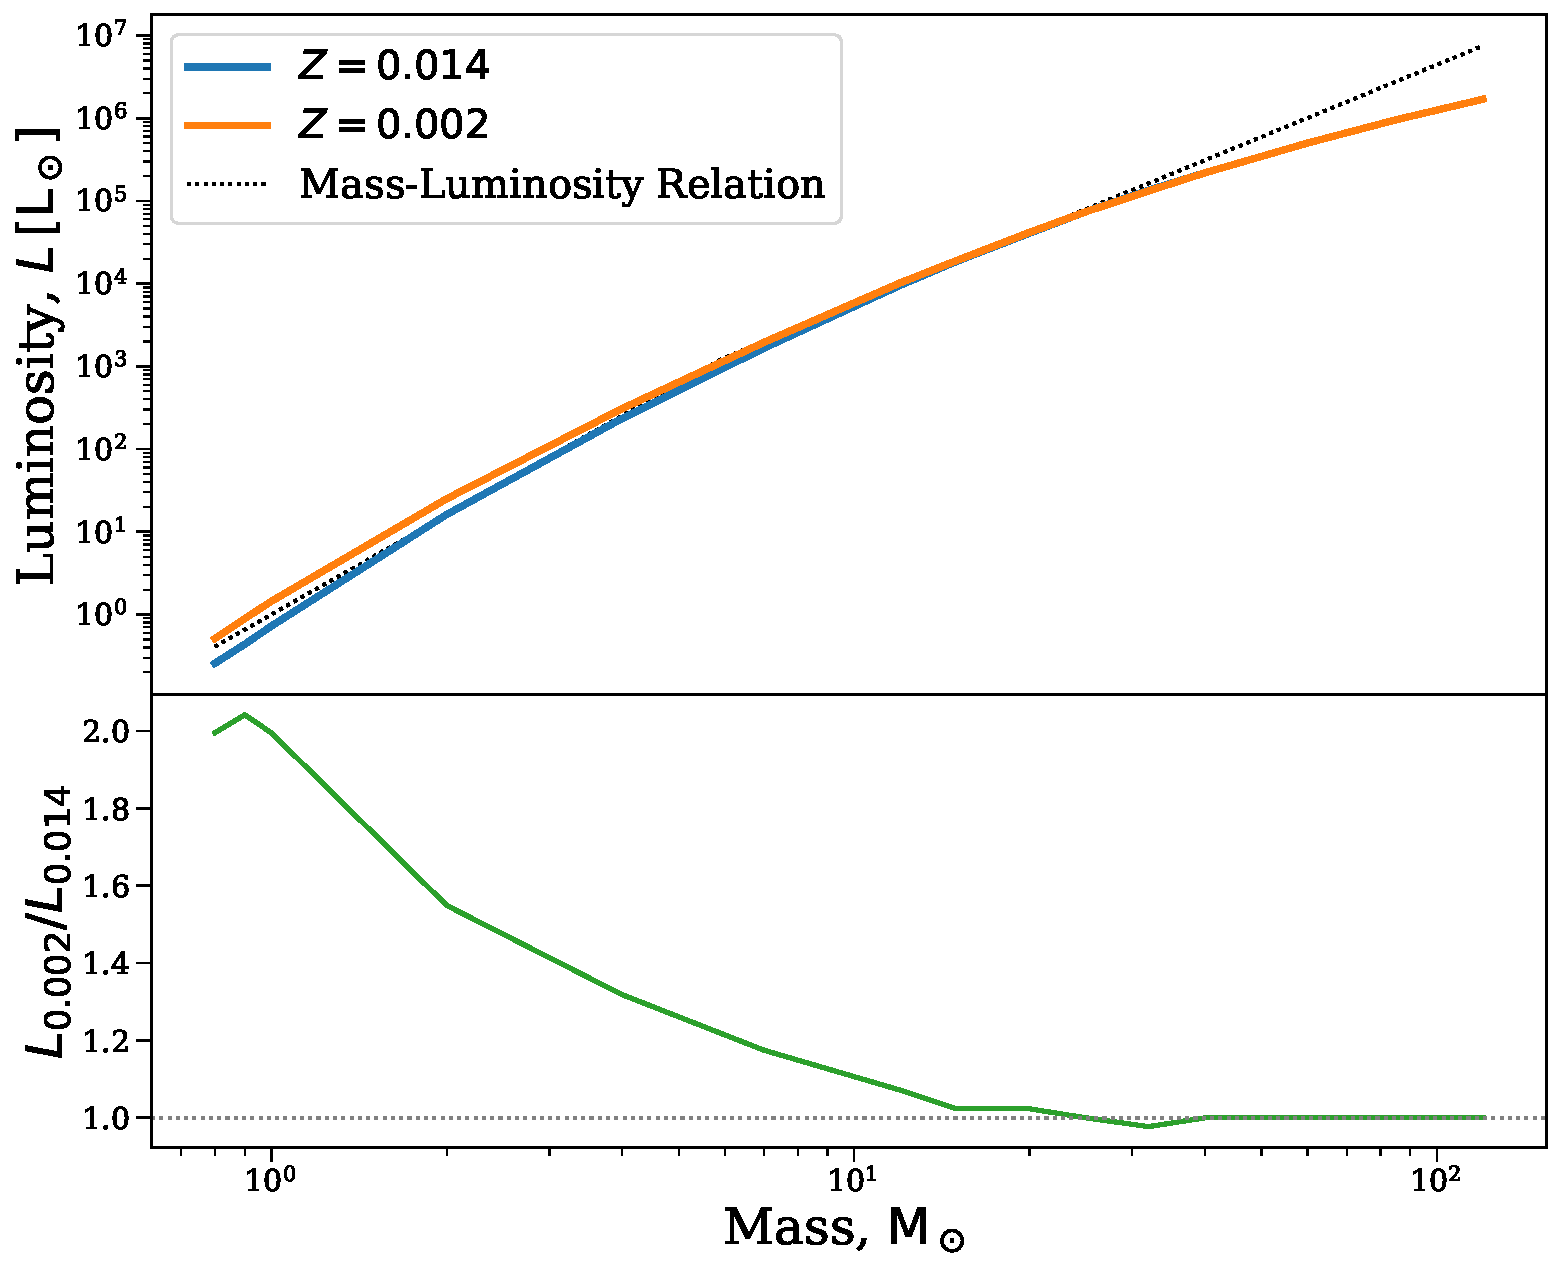
\includegraphics[width=\textwidth]{figures/ml_relation.pdf}
\end{center}

\end{document}

 